\def\year{2015}
%File: formatting-instruction.tex
\documentclass[letterpaper]{article}
\usepackage{float}
\usepackage{aaai}
\usepackage{times}
\usepackage{helvet}
\usepackage{courier}
\usepackage{graphicx}
\usepackage{subfigure}
\usepackage{amsmath}
\usepackage{cases}
\usepackage{multirow}
\usepackage{array}
\usepackage{amssymb}
\usepackage{color}
\frenchspacing
\setlength{\pdfpagewidth}{8.5in}
\setlength{\pdfpageheight}{11in}
\pdfinfo{
/Title (LSH-Draft)
/Author (Put All Your Authors Here, Separated by Commas)}
\setcounter{secnumdepth}{0}  
 \begin{document}
% The file aaai.sty is the style file for AAAI Press 
% proceedings, working notes, and technical reports.
%

% edit & comments
\newcommand{\xhedit}[1]{{\color{blue} #1}}
\newcommand{\xhcomment}[1]{\xhedit{[XH: #1]}}

% math symbols
% influence strength
\newcommand{\ISM}{A}
\newcommand{\IS}{\alpha}

% popularity of story (diffusion speed or activation probability)
\newcommand{\DS}{P}

% number of Activation node
\newcommand{\NActNodes}{N}


\title{Formatting Instructions \\for Authors Using \LaTeX{}}
\author{AAAI Press\\
Association for the Advancement of Artificial Intelligence\\
2275 East Bayshore Road, Suite 160\\
Palo Alto, California 94303\\
}
\maketitle
\begin{abstract}
\begin{quote}
AAAI creates proceedings, working notes, and technical reports directly from electronic source furnished by the authors. To ensure that all papers in the publication have a uniform appearance, authors must adhere to the following instructions. 
\end{quote}
\end{abstract}
%&&&&&&&&&&&&&&&&&&&&&&&&&&&&&&&&&&
\section{Introduction}
Understanding the processes and dynamics of \emph{information diffusion} through networks plays a fundamental role in a variety of domains, such as evaluating the effects of networks in marketing~\cite{domingos:2001,kempe:2003,leskovec:2007a}, monitoring the spread of news, opinions, and scientific ideas via citation networks~\cite{adar:2004,gruhl:2004,leskovec:2005}, and detecting the spread of erroneous information~\cite{dong:2009}.

In practical applications, the underlying diffusion network (e.g. networks on who influenced whom) is often hidden. Therefore, many interesting models have been developed to automatically infer diffusion networks from cascade observations, i.e., timestamps when users post a blog on certain topics or purchase products~\cite{gomez-rodriguez:leskovec:krause:inferring,gomez-rodriguez:balduzzi:schoelkopf:uncovering,yang:zha:mutualExciting,zhou:zha:song:mutualExciting,Wang:Hu:Philip:Li:multiAspect,Daneshmand:Gomez:Song:recovery14,Du:Song:Song:Alex:HeterogeneousInf,Du:Song:Woo:Zha:topicCascade}. 


To be more specific, the diffusion network is usually modeled as a matrix $A=\{\alpha_{u,v}\}$, where $\alpha_{u,v}$ is a parameter as the strength of influence user $u$ has on $v$. Depending on the diffusion model, $\alpha_{u,v}$ can stand for the parameter of the delay distribution for information to propagate from $u$ to $v$ or the probability that $v$ publish a related post given that $u$ has published a post previously. The \emph{Network Inference} problem focuses on discovering the all parameters $\alpha_{u,v}$ from the observed cascades. 



Most previous work on network inference assume that the strength of influence $\alpha_{u,v}$ between $u$ and $v$ remains the same during the whole life of the diffusion processes. We can easily see that this assumption is unrealistic. Consider the propagation of a story in microblog as an example. It is more likely for a user to be influenced by friends to talk about the story when it is popular due to its freshness in the beginning of the propagation. On the contrary, when the story becomes stale and less popular towards the end of its life, it is less likely that one can influence her friends to have interest in it. 


Ignoring the heterogeneity of influence strength in different stages can lead to unsatisfactory solution of the Network Inference problem. Assume that we observe user $v$ posts the same contents immediately after $u$. Existing Network Inference algorithm will treat it as a strong evidence that user $u$ has strong influence on $v$. However, it is also possible that $v$ reposes fast simply because the story is very popular and any of her friends' post will lead to similar rapid response. On the other hand, if the above scenario occurs when the story is not no longer popular, $v$'s rapid response to $u$'s post can be safely treated as strong evidence that $u$ is very influential on $v$. The confusion between strong influence between friends and the popularity of the story leads to the failure in this scenario.  


In this work, we propose to incorporate the heterogeneity of influence strength in different life stage of diffusion process to improve the accuracy of network inference. We design a heuristic referred to as \emph{Life Stage Heuristics} (LSH) that can be easily applied to any existing network inference algorithm. In our LSH, we model the strength of influence as a function of the diffusion life stage $\alpha_{u,v}(t)$ instead of a constant $\alpah_{u,v}$ in previous network inference algorithms.  first approximate the popularity in different life stage by the number of activation. Then, the diffusion rate associated with each edge is  modeled as the multiplication of the popularity of the information in the current stage and the strength of influence between the pair of individuals.     

Recent work has shown that the network inference algorithms are more effective when considering the \emph{heterogeneous} influence such as topic-dependent transmission rates~\cite{Du:Song:Woo:Zha:topicCascade}, heterogenous delay distribution~\cite{Du:Song:Song:Alex:HeterogeneousInf} and multi-aspects multi-pattern cascades~\cite{Wang:Hu:Philip:Li:multiAspect}. However, most previous work ignore the heterogeneity of diffusion speed with respect to the life stage of the cascade. Instead, they assume 

 
Most previous work on network inference assumes that all propagations share the \emph{same} diffusion network. We can easily see that this assumption is unrealistic as the influence between users depends on the topic or the entity under propagation. For example, IT analysts have more influence on others regarding the choice of smart phones, while users tend to trust personal friends as a doctor on medical advices. Moreover, recent work has shown that the network inference algorithms are more effective when considering the \emph{heterogeneous} influence such as topic-dependent transmission rates~\cite{Du:Song:Woo:Zha:topicCascade}, heterogenous delay distribution~\cite{Du:Song:Song:Alex:HeterogeneousInf} and multi-aspects multi-pattern cascades~\cite{Wang:Hu:Philip:Li:multiAspect}. Inferring aspect-specific diffusion networks is a challenging problem.  Naively applying existing network inference algorithms to each aspect-specific cascades independently usually results in unsatisfactory solution. For example, for a network with a hundred nodes, they usually require at least a thousand cascades to achieve accurate inference~\cite{gomez-rodriguez:leskovec:krause:inferring}, while in practice it is unlikely that we can gather this many number of cascades for each topic. 
%&&&&&&&&&&&&&&&&&&&&&&&&&&&&&&&&&&
\section{Empirical analysis}
In this section, we carry out empirical analysis on two real world cascades datasets to show that the assumption of constant influence strength does not hold. We then provide a method to estimate the popularity of the information under propagation empirically from the observed cascades. 

\subsection{Existence of influence strength heterogeneity}
In many network inference models, the influence strength parameter $\alpha_{u,v}$ models the speed of diffusion, namely the time it takes for the information to propagation from user $u$ to $v$.  We empirically estimate the average diffusion speed as the inverse of delay time in two real world cascade datsets, Sina microblog and US Patent to show the heterogeneity of influence strength. \xhcomment{Please add a brief introduction to the datasets.}

The estimation process is as follows: we first normalize the span of each cascade to $[0,1]$ and split the interval into ten bins. We treat each bin as one stage of the diffusion process. We estimate the average diffusion speed in each bin as the inverse of delay time $\frac{1}{\Delta_t}$ using the available explicit following information in the datasets. \xhcomment{What is the unit of y-axis? Is it the diffusion speed after normalization?} The results on two cascades from each dataset is shown in Figure \ref{fig:PatentHetero}. 
\begin{figure}[H]
\subfigure[Cascades of Sina Microblog dataset]{\centerline{
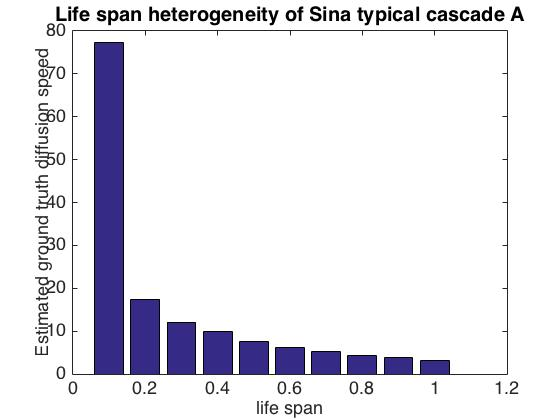
\includegraphics[width=0.55\linewidth]{figures/SinaA.jpg}
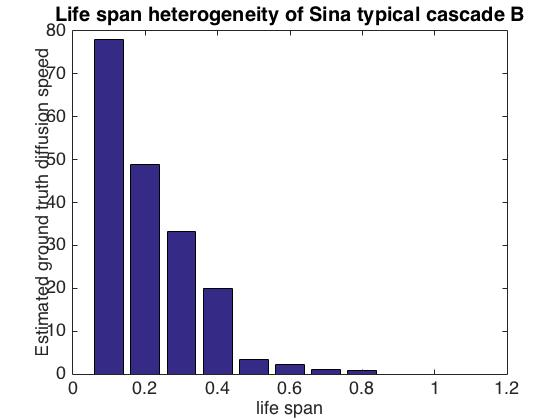
\includegraphics[width=0.55\linewidth]{figures/SinaB.jpg}}}
\subfigure[Cascades of U.S. Patent dataset]{\centerline{
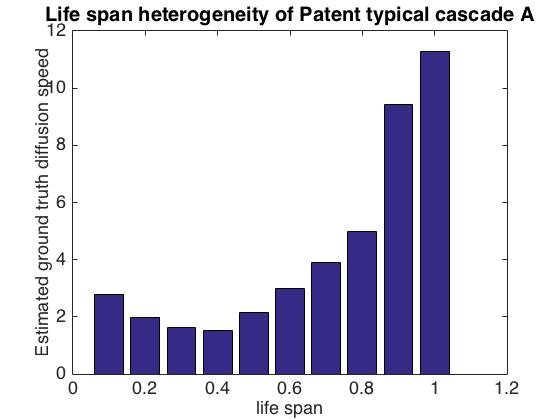
\includegraphics[width=0.55\linewidth]{figures/PatentA.jpg}
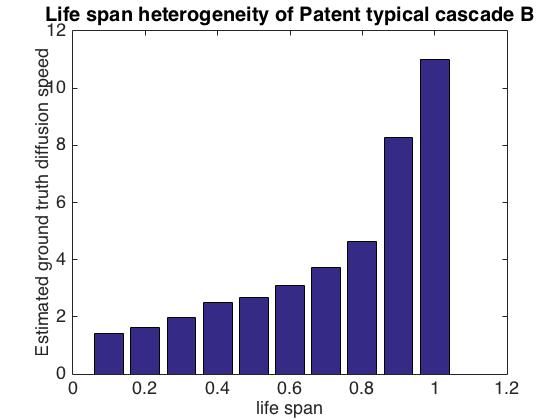
\includegraphics[width=0.55\linewidth]{figures/PatentB.jpg}}}
\caption{The diffusion speed in different stages of diffusion process in two real world datasets. \xhcomment{Could we provide name for each cascade? link the story in microblog and the porduction in patent}}\label{fig:PatentHetero}
\end{figure}

The results clearly demonstrate the deviation from the assumption of constant diffusion speed. Another interesting observation is that the how the diffusion speed depends on the diffusion stages varies dramatically over different cascades and datasets. For the microblog datasets, usually the diffusion speed decrease when the story under propagation becomes stale and less interesting as time elapses. On the contrary, in the patent datsets, newly invented product gradually gains popularity leading to increment in the diffusion speed. 

%It implies that assuming particular functional form of the popularity for all cascades may lead to inaccurate estimation. As a result, we propose to represent the cascade popularity $\DS(t)$ as a piece-wise constant function. Assume we split the normalized span of the cascade into $k$ bins with $t_0=0 < t_1 < \ldots < t_K = 1$. We have $\DS(t) = \DS_i$ if $t\in[t_{i-1}, t_i]$.

%We make an interesting analysis of message's diffusion speed on 2 real world datasets: Sina microblog and U.S. patent. We normalize the activation times with Min-Max method and divide the time length of cascade into several periods.
%As diffusion speed is unmeasurable, we compute the $\frac{1}{\overline{\Delta t}}$ in each life span that is proportion to the ground truth diffusion speed. As in Figure \ref{fig:PatentHetero}, the maximum of $\frac{1}{\overline{\Delta t}}$ reaches 80 in Sina and about 12 in Patent dataset, while the minimum approaches 0. There is distinct difference of diffusion speed in different life span. However, former algorithms have not taken this into consideration. They assume that the coefficient of $\Delta t$'s distribution which controls diffusion speed does not change with time. We believe the life span heterogeneity is a key point to re-understand network inference problem.

%==========================
\subsection{Approximation popularity with number of activation}
Direct estimation of average diffusion speed requires the diffusion pathway which is usually not available in real world datasets. It is even harder to estimate the average activation probability from observed cascades. As a result, we have to seek approximation for the true popularity for different stages in the diffusion process. In the work, we find the total number of activated nodes in each stage of the diffusion process as a good surrogate for the average diffusion speed or the activation probability as a measure for the popularity level. 

Let $I^c(t)$ be the number of activated nodes in cascades $c$ till time $t$. We approximate the popularity level with the following formula:
$$
\DS^c(t) = (I^c(t+\frac{L}{2}) - I^c(t-\frac{L}{2})) / I^c(1).
$$
That is to say, the estimated popularity level at time $t$ is ratio of nodes activated in the windows of length $L$, $[t-\frac{L}{2}, t+\frac{L}{2}]$. 

We carry out experiments to show that the proposed surrogate popularity level is a valid approximation. We select 80 long cascades in Patent dataset and 50 long cascades in Sina dataset\xhcomment{More details on how you choose the cascades? random? longest?}. For each cascade, we first normalize the time span to $[0,1]$ and split it into $K$ bins\xhcomment{What K did you use?}. The true popularity level is assumed to be constant as the average diffusion speed estimated from the particular cascade. We compare the true popularity level and the surrogate popularity at each activation time $t_a$ by computing the Pearson correlation for each cascade. The distribution on the correlation coefficient on the two datasets are shown in Table \ref{tab:Corre}. More than 60\% cascades and 80\% cascades in Patent and Sina microblog dataset respective have correlation coefficient $r>0.6$ with the true popularity level.   
\xhcomment{This is just my guess of what you are doing? Please check is the description correction?}


%We show the validity of this approach by empirically calculating the correlation. We select 80 long cascades in Patent dataset and 50 long cascades in Sina dataset. As in Table \ref{tab:Corre}, we use Evans's (1996) interpretation for r coefficient to describe the strength of correlation. 65\% of Patent cascades and 90\% of Sina cascades present strong or very stronger correlation. Our approach of calculating activated nodes number can reflect the level of diffusion speed to a large extent.
\begin{table}[H]
\caption{Correlation coefficients between ground truth diffusion speed and the number of activated nodes in time unit.}
\begin{tabular}{c|c|c|c}
 coefficient range & strength & pct. Patent & pct. Sina \\
\hline
.00-.19 & very weak & 0.05 & 0.02\\
.20-.39 & weak & 0.125 & 0.02\\
.40-.59 & moderate & 0.175 & 0.06\\
.60-.79 & strong & 0.3 & 0.08\\
.80-1.0 & very strong & 0.35 & 0.82\\
\end{tabular}\label{tab:Corre}
\end{table}
%&&&&&&&&&&&&&&&&&&&&&&&&&&&&&&&&&&
\section{Proposed algorithm}
In this section, we'll introduce (C)LSH method that aims to improve inferring performance by taking advantage of information about messages' diffusion speed. Note that our methods don't ask for any extra input data other than traditional cascades set. We'll show that our method can be easily incorporated into existing network inference algorithms without adding any computational overhead. Some procedures for optimizing our method will be discussed at the end of this section.
%==========================
\subsection{Data and definitions}
%==========================
\subsection{Incorporation with existing algorithms}
We incorporate our method into 3 existing algorithms: NetRate, ConNie and NetInf. We make several changes to the original algorithms without breaking their main structure.
\begin{itemize}
\item LSH-NetRate
\\The transmission likelihood of an activated node $j$ infecting $i$ depends not only on infection time delay $(t_i-t_j)$ and edge strength $\alpha_{ji}$, but also on the diffusion speed of message $c$ at time $t_j$. Transmission is more likely to occur with high diffusion speed, short infection interval and strong connection of edge.
\\We redefine the transmission rate function by combining edge strength and diffusion speed together, denoted as:
\begin{equation}
g_{ji}(t_j,\alpha_{ji})=\alpha_{ji}*S_p(t_j);
\end{equation}
\\Subsequently, survival analysis functions are:
\begin{itemize}
\item Exponential model:
\begin{numcases}{f(t_i|t_j,g_{ji})=}
g_{ji}*e^{-g_{ji}*(t_i-t_j)}, & if $t_j<t_i$ \nonumber \\
0, & otherwise \nonumber
\end{numcases}
%-------------
\begin{flalign*}
    & \log{S(t_i|t_j,g_{ji})}=-g_{ji}*(t_i-t_j) \nonumber &\\
    & H(t_i|t_j,g_{ji})=g_{ji} &\\
\end{flalign*}
%--------------
\item Power law model:
\begin{numcases}{f(t_i|t_j,g_{ji})=}
\frac{g_{ji}}{\delta}(\frac{t_i-t_j}{\delta})^{-1-g_{ji}}, & if $t_j<t_i$ \nonumber \\
0, & otherwise \nonumber
\end{numcases}
\begin{flalign*}
    & \log{S(t_i|t_j,g_{ji})}=-g_{ji}*log(\frac{t_i-t_j}{\delta}) \nonumber &\\
    & H(t_i|t_j,g_{ji})=g_{ji}\ast \frac{1}{t_i-t_j} &\\
\end{flalign*}
%--------------
\item Rayleigh model:
\begin{numcases}{f(t_i|t_j,g_{ji})=}
g_{ji}(t_i-t_j)e^{-\frac{1}{2} g_{ji} (t_i-t_j)^2}, & if $t_j<t_i$ \nonumber \\
0, & otherwise \nonumber
\end{numcases}
\begin{flalign*}
    & \log{S(t_i|t_j,g_{ji})}=-g_{ji}*\frac{(t_i-t_j)^2}{2} \nonumber &\\
    & H(t_i|t_j,g_{ji})=g_{ji}\ast (t_i-t_j) &\\
\end{flalign*}
%\renewcommand{\multirowsetup}\centering
%\begin{table*}
%\begin{tabular}{p{2cm}<{\leftline}|p{7.5cm}<{\centering}|p{3cm}<{\centering}|p{3cm}<{\centering}}
%\hline  
%\multirow{2}{*}{Model} & Tansmission likelihood & Log survival function & Hazard function\\
%& $f(t_i|t_j,g_{ji})=$ & $\log{S(t_i|t_j,g_{ji})}=$ & $H(t_i|t_j,g_{ji})=$ \\\hline
% & 
%\multirow{2}{*}{\begin{numcases}{f(t_i|t_j,g_{ji})=}
%g_{ji}*e^{-g_{ji}*(t_i-t_j)}, & if $t_j<t_i$ \nonumber \\
%0, & otherwise \nonumber
%\end{numcases}} \\
%\hline 
%\end{tabular}
%\end{table*} 
Note that the computation of $S_p(t_j)$ is finished in pre-processing. $S_p(t_j)$ are constants in inference process which will not affect the survival analysis process. The range of $S_p(t_j)$ is [0,1]. Constraints of the former problem have no change.  
\end{itemize}
%--------------
\item LSH-ConNie
\\ConNie declares a weighted adjacency matrix $A$ each entry of which controls the conditional probability of edge transmission. In our method, transmission probability on an edge depends on diffusion speed of parent node's time($S_p(t_j)$) besides edge weight $A_{ji}$. We define the transmission rate function by combining $S_p(t_j)$ and edge weight, denoted as:
\begin{equation}
g_{ji}(t_j,A_{ji})=A_{ji}*S_p(t_j);
\end{equation}
When inferring the incoming edges of node $i$, the modified likelihood function of $i$ is:
\begin{equation}
\begin{aligned}\label{eq:ConnieUnConvex}
L_{i}(A_{:,i};C) &=\prod_{c\in C;t_i^c<\infty} \bigg[ 1-\prod_{j:t_j \leq t_i}(1-w_{ji}g_{ji}(t_j^c,A_{ji}))\bigg] \\
 &\ast \prod_{c\in C;t_i^c=\infty} \prod_{j:t_j^c<\infty}(1-g_{ji}(t_j^c,A_{ji}))
\end{aligned}
\end{equation}
We have to transform this into a convex optimization problem as the way ConNie did. Similarly, we redefine the variables $B_{ji}^c$ and $\gamma_c$. Note that as we incorporate $S_p(t_j)$ into $B_{ji}^c$, the new defined variable $B^C$ is more than just a $N*N$ matrix ($N$ is the number of nodes in ground truth network). There are $|C|$ of $N*N$ matrix to be estimated in $B^C$, the size of which will change with the cascades amount.
\begin{eqnarray} 
&B_{ji}^c=1-g_{ji}(t_j^c,A_{ji})\\
&\gamma_c=1-\prod_{j:t_j \leq t_i}(1-w_{ji}\ast g_{ji}(t_j^c,A_{ji})) \label{eq:ConnieGamma}
\end{eqnarray}
Our method makes no change to the constraints of $B_{ji}^c$ and $\gamma_c$ as the range of $S_p(t_j)$ is [0, 1], too. The objective problem becomes:
\begin{equation}
\max_{\gamma_c,B^C(:,i)}\prod_{c\in C;t_i^c<\infty} \gamma_c \ast \prod_{c\in C;t_i^c=\infty} \prod_{j:t_j^c<\infty}B_{ji}^c 
\end{equation}
\begin{eqnarray}
& subject \quad to:\nonumber \\
& 0 \leqslant B_{ji}^c \leqslant 1 \quad \forall j \nonumber \\
& 0 \leqslant \gamma_c \leqslant 1 \quad \forall c \nonumber \\
& \gamma_c+\prod_{j:t_j \leq t_i}\bigg(1-w_{ji}\ast \big(1-B_{ji}^c\big)\bigg) \leqslant 1 \quad \forall c. \nonumber 
\end{eqnarray}
Negative logarithm of the objective problem is shown in Eq.\ref{eq:ConnieObj}, in which $\hat{\gamma_c}=\log{\gamma_c}$ and $\hat{B_{ji}^c}=\log{B_{ji}^c}$:
\begin{equation}\label{eq:ConnieObj}
\min_{\gamma_c,B^C(:,i)}-\sum_{c\in C;t_i^c<\infty} \hat{\gamma_c} - \sum_{c\in C;t_i^c=\infty} \sum_{j:t_j^c<\infty}\hat{B_{ji}^c} 
\end{equation}
\begin{eqnarray}
& subject \quad to:\nonumber \\
& \hat{B_{ji}^c} \leqslant 0 \quad \forall j \nonumber \\
& \hat{\gamma_c} \leqslant 0 \quad \forall c \nonumber \\
& \log{\bigg[e^{\hat{\gamma_c}}+\prod_{j:t_j \leq t_i}\bigg(1-w_{ji}\ast \big(1- e^{\hat{B_{ji}^c}} \big)\bigg) \bigg] \leqslant 0} \quad \forall c. \nonumber 
\end{eqnarray}
The problem defined in Eq.\ref{eq:ConnieObj} is convex on its variables $\gamma_c$ and $B^C(:,i)$. 
In order to transform Eq.\ref{eq:ConnieUnConvex} into convex problem, we have got more variables which might add to the computation burden. We'd like to propose a compromise to reduce variables amount when cascades number is large. We skip the $S_p$ property of the second part of Eq.\ref{eq:ConnieUnConvex}, which is:
\begin{equation}
\begin{aligned}\label{eq:ConnieUnConvex}
L_{i}(A_{:,i};C) &=\prod_{c;t_i^c<\infty} \bigg[ 1-\prod_{j:t_j \leq t_i}(1-w_{ji}*g_{ji}(t_j^c,A_{ji}))\bigg] \\
 &\ast \prod_{c;t_i^c=\infty} \prod_{j:t_j^c<\infty}(1- \underline{A_{ji}})
\end{aligned}
\end{equation}
By this way, we can declare $B_{ji}^{'}=1-A_{ji}$ without considering its variance in different cascades, while $\gamma_c$ stays as it is in Eq.\ref{eq:ConnieGamma}. The number of variables reduces to $N*N+|C|$ as we demand.
%--------------
\item LSH-NetInf
\\NetInf algorithm considers only the infection time interval in transmission probability function. We incorporate LSH method into NetInf by combining diffusion speed with the original transmission probability. Basically, the redefined $P_c(u,v)$ of exponential model and power-law model is:
\begin{eqnarray}
\hat{P_c}(u,v)=\alpha S_p(t_u)*e^{-\frac{t_v-t_u}{\alpha S_p(t_u)}} \nonumber \\
\hat{P_c}(u,v)=(\alpha S_p(t_u)-1)\frac{1}{(t_v-t_u)^{\alpha S_p(t_u)}} \nonumber
\end{eqnarray} 
NetInf does not consider all possible propagation trees but only the most likely one. The modified likelihood in LSH-NetInf of all cascades with the maximum weighted propagation tree is:
\begin{equation}
\begin{aligned}
P(C|G)&=\prod_{c\in C} \sum_{T\in \mathcal{T}_c(G)}P(c|T) \\
&\approx \prod_{c\in C} \max_{T\in \mathcal{T}_c(G)}P(c|T) \nonumber \\
&\approx \beta^q \varepsilon^{q'} (1-\varepsilon)^{s+s'}\prod_{(u,v)\in E_{T}}\hat{P_c}(v,u)
\end{aligned}
\end{equation}
As noted in NetInf paper, $q$ is network edges number and $q'$ is $\varepsilon$-edges number in $T$; $s$ and $s'$ refer to those that did not transmit respectively.
Note that our method just affects the pairwise transmission probability of the original NetInf algorithm without breaking its main structure or imposing extra computation burden.
\end{itemize} 
%==========================
\subsection{Optimization methods}
\subsubsection{Clustering cascades}

\subsubsection{Dealing with root node}
%&&&&&&&&&&&&&&&&&&&&&&&&&&&&&&&&&&
\section{Experiments}
Experiments for LSH and CLSH are performed to evaluate their abilities in improving network inference algorithms' performance. We mainly focus on 3 existing algorithms: NetRate, ConNie , NetInf, on which we apply LSH and CLSH method respectively. 
%==========================
\subsection{Experiments on synthetic dataset}
Synthetic networks of 256 nodes are generated from Kronecker model with parameter matrix [0.5 0.5; 0.5 0.5]. At the beginning of each cascade, root node is selected randomly and recorded as $t=0$. Pairwise edge weights are sampled from $U(0,1)$. The larger the value of edge weight, the higher the probability of transmitting a message between this pair of nodes.  Once a node is infected, it begins to infect the adjacent nodes. Each activated node infects its neighbors with probabilities generated from transmission likelihood function( Exponential model). The diffusion proceeds iteratively until time window $T$, which is set at 10.
\\ Measures in this paper are AUC(Area under Precision-Recall curve) and maximum $F_1$ score. $F_1$ score is the harmonic mean of precision and recall while we consider the maximum value in evaluation.
\\ When generating synthetic cascade data, we use the piecewise function $S_p(t_j)$ to control life span heterogeneity. Value of $S_p(t_j)$ implies the diffusion speed of message in $t_j$. Large deviation in $S_p(t_j)$ causes strong heterogeneity. In this part, $S_p(t_j)$ is set as [0.03 0.9 0.07 0 0]. (time window $T=10$ as noted) When $T_j=3.2$, $S_p(t_j)=0.9$; when $T_j=5.9$, $S_p(t_j)=0.07$, etc.
\\\textbf{Performance vs. cascade number.} We make experiments of LSH-NetRate/LSH-ConNie/LSH-NetInf. By applying LSH method, the performance of network inference improves comparing with their original algorithms, as shown in Table \ref{tab:synLSHCASf1} and \ref{tab:synLSHCASAUC}. Figure \ref{fig:synLSHpr} plots the Precision-Recall curve of LSH-NetRate/LSH-ConNie/LSH-NetInf method. Our methods make distinct improvement.
\begin{table}[H]
\caption{Max $F_1$ score of LSH-NetRate/LSH-ConNie/LSH-NetInf vs. casNum}
\begin{tabular}{c|c|c|c}
 & casNum 300 & casNum 600 & casNum 900 \\
\hline
NetRate & 0.6742 & 0.7913 & 0.8161\\
LSH-NetRate & 0.7251 & 0.8210 & 0.8425\\
\hline
ConNie & 0.7500 & 0.7526 & 0.7905\\
LSH-ConNie & 0.7653 & 0.7734 & 0.8138\\
\hline
NetInf & 0.5927 & 0.6799 & 0.7360\\
LSH-NetInf & 0.6018 & 0.6997 & 0.7446
\end{tabular}\label{tab:synLSHCASf1}
\end{table}
%--------------
\begin{table}[H]
\caption{Area under PR curve of LSH-NetRate/LSH-ConNie/LSH-NetInf vs. casNum}
\begin{tabular}{c|c|c|c}
 & casNum 300 & casNum 600 & casNum 900 \\
\hline
NetRate & 0.4794 & 0.6299 & 0.6858\\
LSH-NetRate & 0.5573 & 0.6892 & 0.7805\\
\hline
ConNie & 0.6899 & 0.7424 & 0.7985\\
LSH-ConNie & 0.6916 & 0.7657 & 0.8334\\
\hline
NetInf & 0.3801 & 0.4638 & 0.5754\\
LSH-NetInf & 0.4186 & 0.5421 & 0.5764
\end{tabular}\label{tab:synLSHCASAUC}
\end{table}
\begin{figure*}
\centerline{
\subfigure[LSH-NetRate]{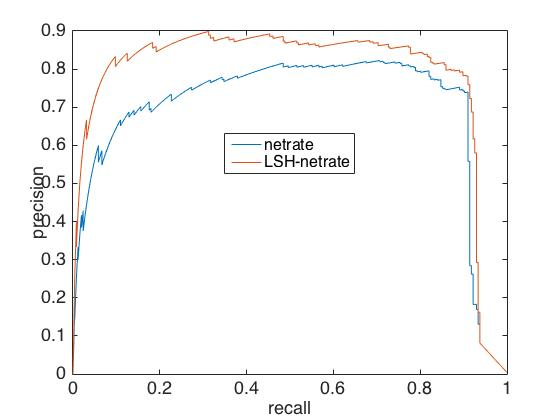
\includegraphics[width=0.35\linewidth]{figures/PR900.jpg}}
\subfigure[LSH-ConNie]{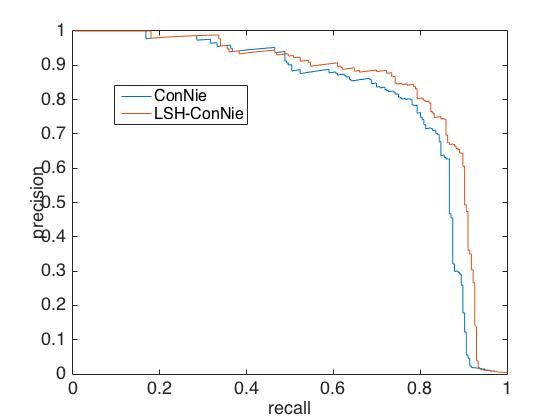
\includegraphics[width=0.35\linewidth]{figures/Connie900.jpg}}
\subfigure[LSH-NetInf]{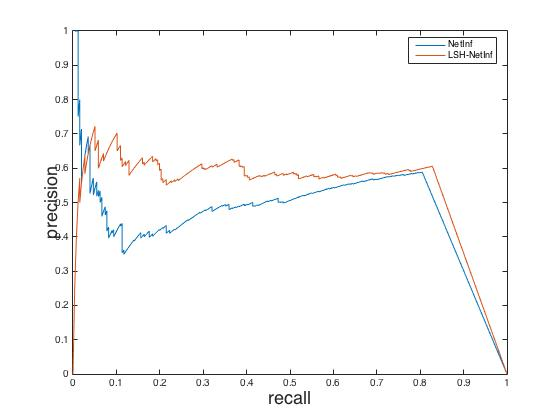
\includegraphics[width=0.35\linewidth]{figures/NetInfPR.jpg}}}
\caption{Precision-Recall curve of LSH-NetRate/LSH-ConNie/LSH-NetInf method }\label{fig:synLSHpr}
\end{figure*}
%--------------
\textbf{Performance vs. heterogeneity strength.} We generate synthetic cascades with various heterogeneity strength, as shown in Table \ref{tab:Spfunction}. The level of standard deviation depicts the strength of heterogeneity. Experiments in Figure \ref{fig:Hete} show that our method gains larger advantage to original NetRate as standard deviation of $S_p$ increases.
\begin{table}[H]
\caption{4 types of Sp function with different standard deviation.}
\begin{tabular}{c|c|c}
 & Sp function & standard deviation \\
\hline
1 & [0.2 0.2 0.2 0.2 0.2] & 0\\
2 & [0.2 0.4 0.3 0.05 0.05] & 0.1541\\
3 & [0.1 0.6 0.3 0 0] & 0.2549\\
4 & [0.03 0.9 0.07 0 0] & 0.3924
\end{tabular}\label{tab:Spfunction}
\end{table}
\begin{figure}[H]
\centerline{
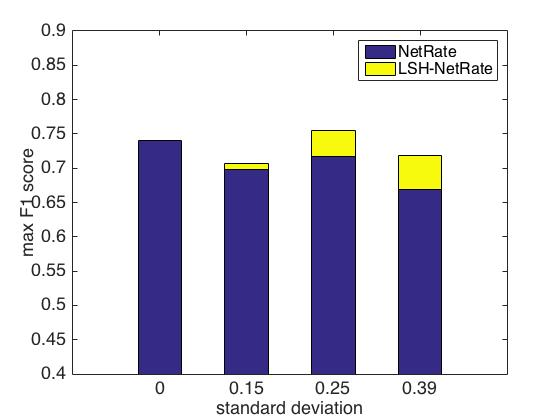
\includegraphics[width=0.75\linewidth]{figures/HeteroStrength.jpg}}
\caption{Experiments on different heterogeneity strength. }\label{fig:Hete}
\end{figure}
%--------------
\textbf{Setting of $lag$.} $lag$ is half the length of sliding window around target time stamp that can affect the estimation of $S_p$. We run our methods with 4 different $lag$ settings separately, results are shown in Figure \ref{fig:SetLAG}. We can see that their differences are slight as we change $lag$'s value. But LSH method performs better with $lag$ set around 10\% of T.
\begin{figure}[H]
\centerline{
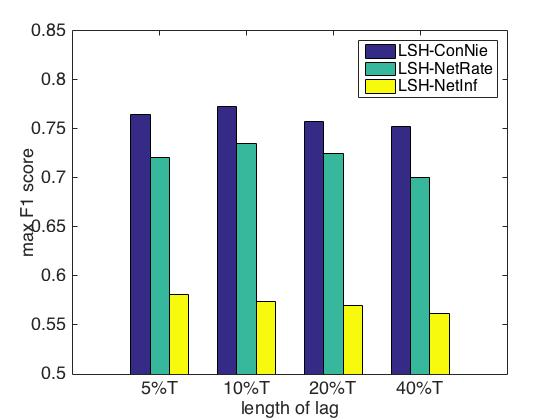
\includegraphics[width=0.75\linewidth]{figures/SettingLAG.jpg}}
\caption{Experiments of different lag values. }\label{fig:SetLAG}
\end{figure}
%--------------
\textbf{Experiments of CLSH method.}
CLSH method attempts to cluster cascades so that cascades in the same group have similar $S_p(t_j)$. In this part, we use 3 types of $S_p(t_j)$ functions: [0.1 0.8 0.1 0 0] / [0.8 0.2 0 0 0] / [0 0 0 0.2 0.8]. Before simulating a cascade, we randomly choose one of this three to be the specific $S_p$ function of this cascade.  
\\\textbf{Performance of CLSH vs. cascade number.} We make experiments of CLSH-NetRate/CLSH-ConNie/CLSH-NetInf methods on synthetic cascades with multiply heterogeneity functions. As shown in Table \ref{tab:synCLSHCASf1} and \ref{tab:synCLSHCASAUC}, our methods outperform the original algorithms on max $F_1$ score and $AUC$. 
\begin{table}[H]
\caption{Max $F_1$ score of CLSH-NetRate/CLSH-ConNie/CLSH-NetInf vs. casNum}
\begin{tabular}{c|c|c|c}
 & casNum 300 & casNum 600 & casNum 900 \\
\hline
NetRate & 0.7124 & 0.7222 & 0.7254\\
CLSH-NetRate & 0.7256 & 0.7425 & 0.7414\\
\hline
ConNie & 0.7296 & 0.7531 & 0.7619\\
CLSH-ConNie & 0.7474 & 0.7520 & 0.7692\\
\hline
NetInf & 0.6727 & 0.7133 & 0.7316\\
CLSH-NetInf & 0.6886 & 0.7314 & 0.7489
\end{tabular}\label{tab:synCLSHCASf1}
\end{table}
%---------------
\begin{table}[H]
\caption{Area under PR curve of CLSH-NetRate/CLSH-ConNie/CLSH-NetInf vs. casNum}
\begin{tabular}{c|c|c|c}
 & casNum 300 & casNum 600 & casNum 900 \\
\hline
NetRate & 0.5243 & 0.5445 & 0.5894\\
CLSH-NetRate & 0.5771 & 0.6527 & 0.6582\\
\hline
ConNie & 0.7006 & 0.7449 & 0.7612\\
CLSH-ConNie & 0.7194 & 0.7600 & 0.7602\\
\hline
NetInf & 0.4079 & 0.4248 & 0.5138\\
CLSH-NetInf & 0.4319 & 0.4402 & 0.5268
\end{tabular}\label{tab:synCLSHCASAUC}
\end{table}
\textbf{Setting of $k$.} As shown in Figure \ref{fig:SetK}, clustering cascades into 3 $\sim$ 4 groups produces higher accuracy.
\begin{figure}[H]
\centerline{
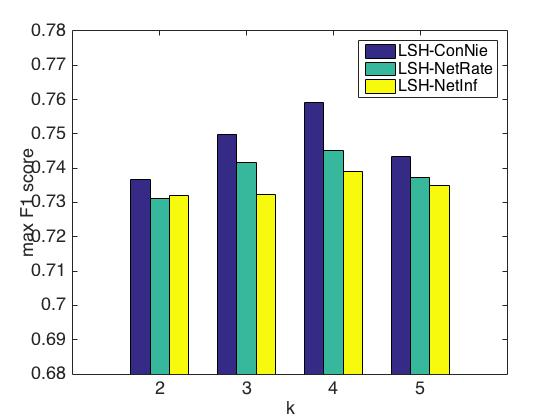
\includegraphics[width=0.75\linewidth]{figures/SettingK.jpg}}
\caption{Experiments of different k values. }\label{fig:SetK}
\end{figure}
%==========================
\subsection{Experiments on real world dataset}
We use \emph{U.S. patent dataset} by \emph{the National Bureau of Economic Research} to test (C)LSH method. The dataset spans 25 years from 1975 to 1999, containing 16,522,438 citations. Inventors of patents cite their sources. Therefore, we take inventors as the entities of network and follow the citations to reveal information flow. Note that we remove all self-loops in patent data, which happen when inventors cite their own previous works. By ranking inventors according to their activity, we have 147 most active inventors to form the ground truth network. We extract 150/250/350/450 transmission trees for cascade information. Experiments of (C)LSH-NetRate, (C)LSH-ConNie, (C)LSH-NetInf are made on this dataset. 
\\For real world dataset, the lengths of cascades differ a lot. We apply Min-Max Normalization to activation times in each cascade separately. Cascades' length is 1 after transformation.
\begin{itemize}
\item (C)LSH-NetRate
\\ \textbf{Performance vs. cascade number. }From Table \ref{tab:rwdLSHnetrateCASf1} we can see improvement by applying LSH method to NetRate on various data scale. Increasing $k$ in some occasions can help improve accuracy.
\begin{table}[H]
\caption{Real data: Max $F_1$ score of NetRate/  LSH-NetRate/ CLSH-NetRate vs. casNum}
\begin{tabular}{c|c|c|c|c}
 & cas 150 & cas 250 & cas 350 & cas 450 \\
 \hline
 NetRate & 0.5915 & 0.6110 & 0.6418 & 0.6667 \\
 LSH-NetRate & 0.6324 & 0.6364 & 0.6817 & 0.6975 \\
 CLSH-k 3 & 0.6328 & 0.6431 & 0.6731 & 0.6997 \\
 CLSH-k 5 & 0.6324 & 0.6360 & 0.6752 & 0.7121
\end{tabular}\label{tab:rwdLSHnetrateCASf1}
\end{table}
%--------------
\item (C)LSH-ConNie
\\ \textbf{Performance vs. cascade number.} LSH method outperforms ConNie notably as shown in Table \ref{tab:rwdLSHconnieCASf1}. Furthermore, applying CLSH to cluster similar cascades extends the performance advantage over original ConNie method.
\begin{table}[H]
\caption{Real data: Max $F_1$ score of ConNie/  LSH-ConNie/ CLSH-ConNie vs. casNum}
\begin{tabular}{c|c|c|c|c}
 & cas 150 & cas 250 & cas 350 & cas 450 \\
 \hline
 ConNie & 0.5702 & 0.6127 & 0.6412 & 0.6788 \\
 LSH-ConNie & 0.8125 & 0.8222 & 0.8532 & 0.8673 \\
 CLSH-k 3 & 0.8249 & 0.8298 & 0.8502 & 0.8733 \\
 CLSH-k 5 & 0.8140 & 0.8218 & 0.8561 & 0.8581
\end{tabular}\label{tab:rwdLSHconnieCASf1}
\end{table}
%--------------
\item (C)LSH-NetInf
\\ \textbf{Performance vs. cascade number.} Table \ref{tab:rwdLSHnetinfCASf1} and \ref{tab:rwdLSHnetinfCASauc} present the AUC and maximum $F_1$ score results of our methods and NetInf algorithm. In all cases, our methods perform better than NetInf. When including more cascades, the complexity increases. Proper increment of $k$ may lead to higher performance.
\begin{table}[H]
\caption{Real data: Max $F_1$ score of NetInf/  LSH-NetInf/ CLSH-NetInf vs. casNum}
\begin{tabular}{c|c|c|c|c}
 & cas 150 & cas 250 & cas 350 & cas 450 \\
 \hline
 NetInf & 0.5284 & 0.5382 & 0.5779 & 0.5981 \\
 LSH-NetInf & 0.7604 & 0.7762 & 0.7993 & 0.7932 \\
 CLSH-k 3 & 0.7757 & 0.7902 & 0.8000 & 0.7938 \\
 CLSH-k 5 & 0.7833 & 0.7762 & 0.8129 & 0.8062
\end{tabular}\label{tab:rwdLSHnetinfCASf1}
\end{table}
\begin{table}[H]
\caption{Real data: AUC of NetInf/ LSH-NetInf/ CLSH-NetInf vs. casNum}
\begin{tabular}{c|c|c|c|c}
 & cas 150 & cas 250 & cas 350 & cas 450 \\
 \hline
 NetInf & 0.7860 & 0.7919 & 0.8160 & 0.8292 \\
 LSH-NetInf & 0.9413 & 0.9393 & 0.9410 & 0.9429 \\
 CLSH-k 3 & 0.9502 & 0.9473 & 0.9418 & 0.9436 \\
 CLSH-k 5 & 0.9547 & 0.9393 & 0.9490 & 0.9506
\end{tabular}\label{tab:rwdLSHnetinfCASauc}
\end{table}
\end{itemize}
%&&&&&&&&&&&&&&&&&&&&&&&&&&&&&&&&&&
\section{Conclusions}
%&&&&&&&&&&&&&&&&&&&&&&&&&&&&&&&&&&
\bibliographystyle{aaai}
\bibliography{misc,names,conferences,theory_submodular,theory_InfMax,ml_NetworkInference,ml_TopicModel,ml_NetworkModel,optimization}

\end{document}
